Была предпринята попытка замерить время исполнения всех 24 вариаций алгоритмов на следующих операциях:

\begin{itemize}
\item Генерация пары ключей (публичный-приватный)
\item Вычисления хэш-значения
\item Электронная подпись сообщения
\item Верификация сообщения
\item Время работы Proof of Work
\item Время майна одного блока
\end{itemize}

Замеры проводились при помощи модуля \emph{time} в Python. Дальнейший анализ и
построение графиков происходило в среде \emph{Jupyter Notebook} с
использованием модуля \underline{matplotlib}.

\begin{figure}
    \centering
    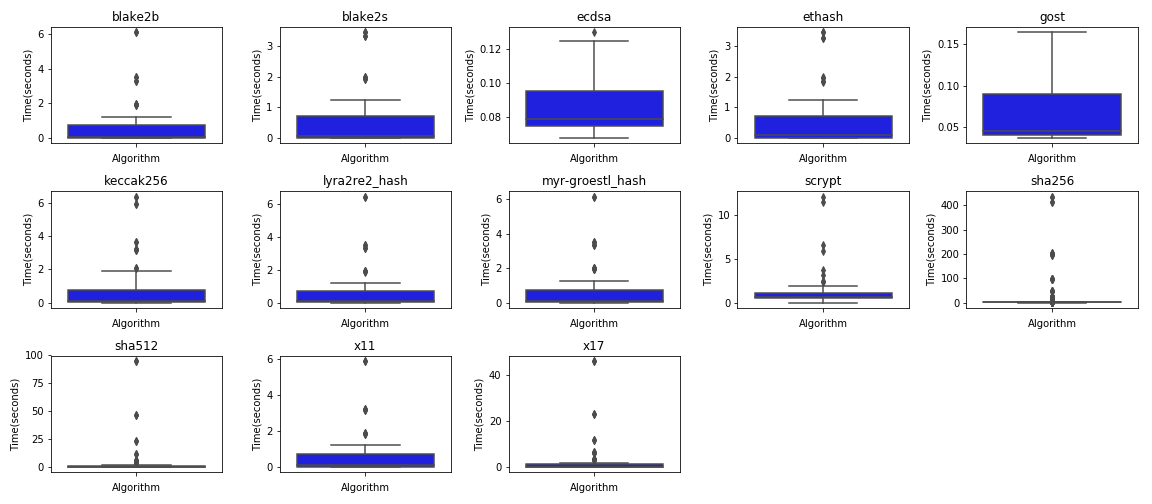
\includegraphics[width=\textwidth]{./images/boxes}
    \caption{Box-plot'ы для распределения алгоритмов по времени}
\end{figure}

Далее были построены гистограммы распределения времени выполнения для
алгоритмов цифровой подписи, разделяя их на вышеперечисленные процессы (Рис. \ref{dss}):

\begin{figure}[h]
    \centering
    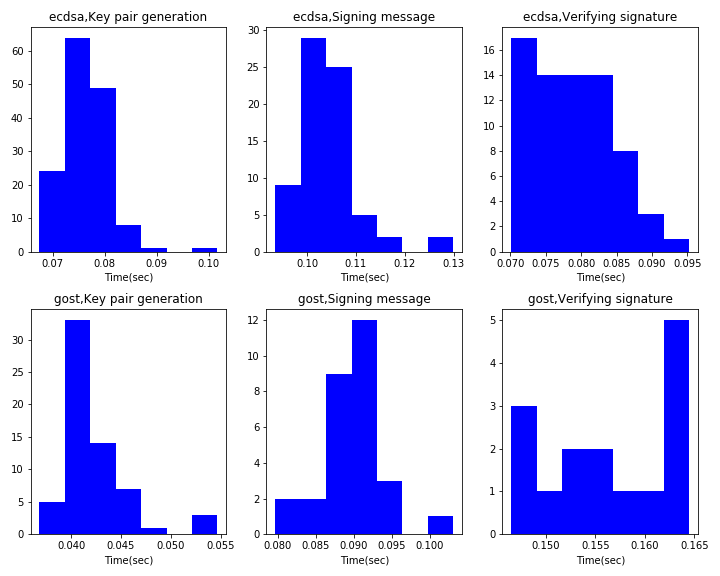
\includegraphics[width=0.68\textwidth]{./images/hists_dss}
    \caption{Распределение времени выполнения среди алгоритмов цифровой подписи}\label{dss}
\end{figure}

И, аналогичные данные быи построены для алгоритмов хэширования (Рис. \ref{hash}):

\begin{figure}
    \centering
    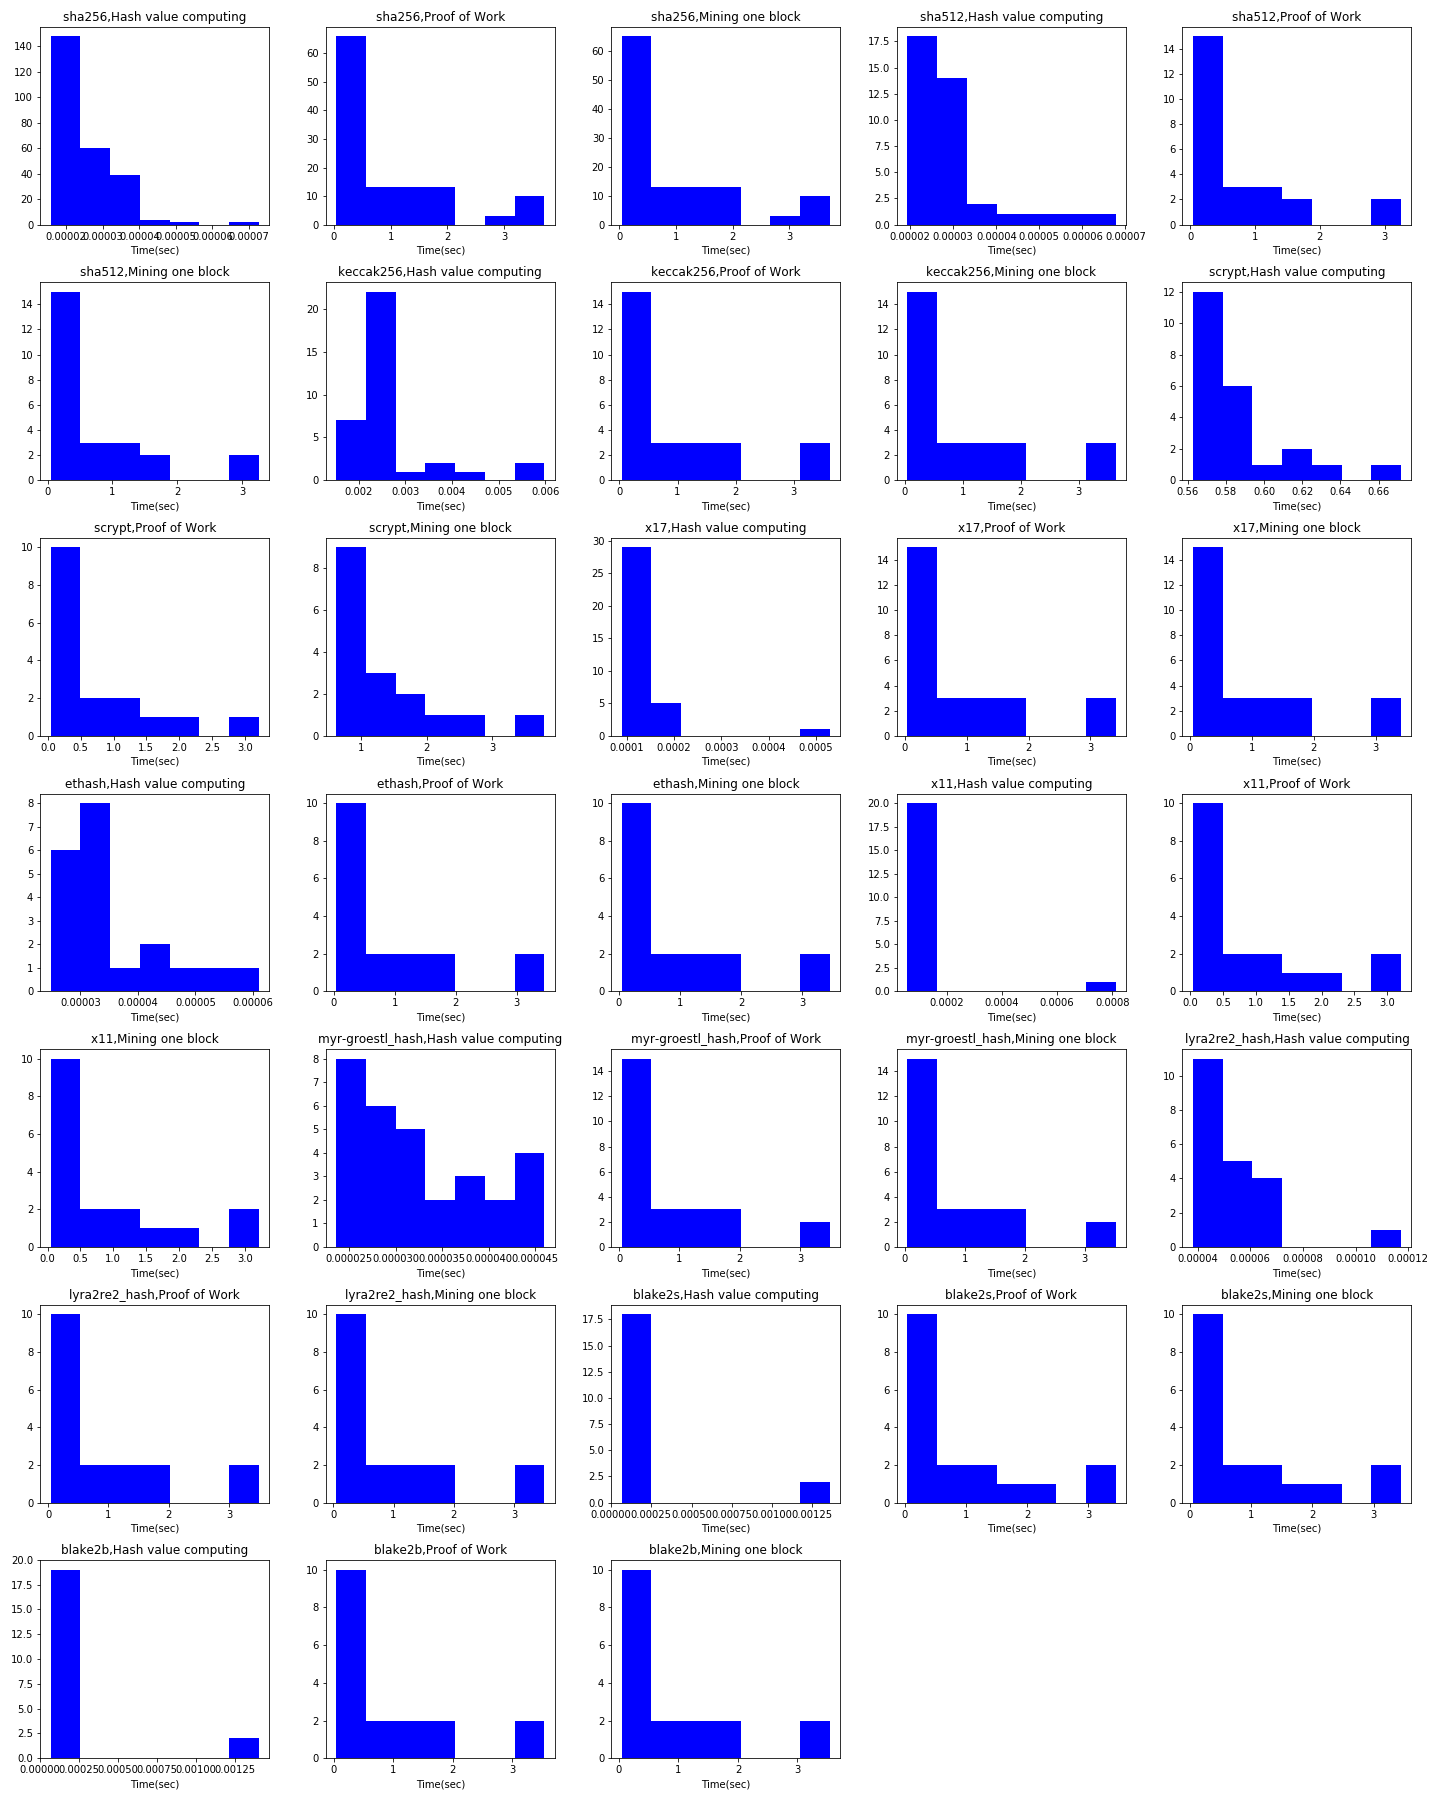
\includegraphics[width=\textwidth]{./images/hists_hashing}
    \caption{Распределение времени выполнения среди алгоритмов хэширования}\label{hash}
\end{figure}



